\documentclass{article}
\usepackage[utf8]{inputenc}
\usepackage[T1]{fontenc}
\usepackage[top=2cm,bottom=2cm,left=3cm,right=3cm]{geometry}
\usepackage{hyperref}
\usepackage{amsmath,amsfonts,amssymb,amsthm}
\usepackage{graphicx}
\usepackage[dvipsnames]{xcolor}

\renewcommand{\figurename}{Rysunek}


\begin{document}
	\title{ \LARGE \textsc{Bazy danych}
		\\ [5.5cm]
		\huge \textbf{\uppercase{Baza danych Geeks \& Dragons}}
		\\ [0.5cm]
		\large \textbf{\uppercase{Dokumentacja}}
		%\\ [0.5cm]
		%\normalsize \today \vspace*{20\baselineskip}
		}
	\date{}
	\maketitle
	\vspace{7.5cm}
	
	\begin{center}
	\author{
		Szymon Malec, 262276 \\
		Adam Wrzesiński, 262317\\
		Michał Wiktorowski, 262330 \\
		Weronika Zmyślona, 262284 \\
		\vspace{0.5cm}
		Politechnika Wrocławska \\
		Wydział Matematyki - Matematyka Stosowana}
	\end{center}
	
	\thispagestyle{empty}
	
	\newpage\thispagestyle{empty}
	\mbox{}
	
	\setcounter {page}{1}
	
	\tableofcontents
	
	\newpage
	\section{Wstęp}
	Niniejsza dokumentacja przedstawia proces tworzenia bazy danych sklepu Geeks \& Dragons w ramach projektu na zaliczenie z kursu Bazy Danych z 2023 roku. Zadanie polegało na wysymulowaniu danych, jakie mogłyby się pojawić w bazie przykładowego sklepu, mającego w ofercie gry nieelektroniczne, który dodatkowo prowadzi wypożyczalnię gier oraz organizuje turnieje. Projekt został wykonany z~wykorzystaniem języka programownaia Python.\\
	
	\noindent Pierwszą częścią projektu było wykonanie schematu bazy danych, a następnie wygenerowanie losowych danych. Uzyskane dane należało eksportować do bazy i umieścić na serwerze za pomocą biblioteki SQLAlchemy. Kolejna część polegała na przeprowadzeniu analizy danych z wysymulowanego zbioru i~przedstawienie jej w formie raportu. Ponadto został opisany przebieg normalizacji bazy danych do postaci EKNF. 
	
	\section{Schemat bazy danych}
	Schemat bazy danych (Rysunek 1.) uwzględnia 8 tabel przechowujących nastepujące informacje:
	\begin{itemize}
		\setlength{\itemsep}{-2pt}
		\item \textbf{cusomer} – dane dotyczące klientów sklepu,
		\item \textbf{staff} – dane dotyczące pracowników sklepu,
		\item \textbf{games\textunderscore for\textunderscore sale} – dane dotyczące gier dostępnych na sprzedaż,
		\item \textbf{games\textunderscore to\textunderscore rent} – dane dotyczące gier dostępnych do wypożyczenia,
		\item \textbf{sale} – dane na temat sprzedaży gier,
		\item \textbf{rental} – dane na temat wypożyczeń gier,
		\item \textbf{competition} – dane dotyczące organizownych turniejów,
		\item \textbf{competition\textunderscore results} – dane dotyczące osiągnietych wyników przez uczestników turniejów.
	\end{itemize}
	
	\begin{figure}[!h]
		\centering
		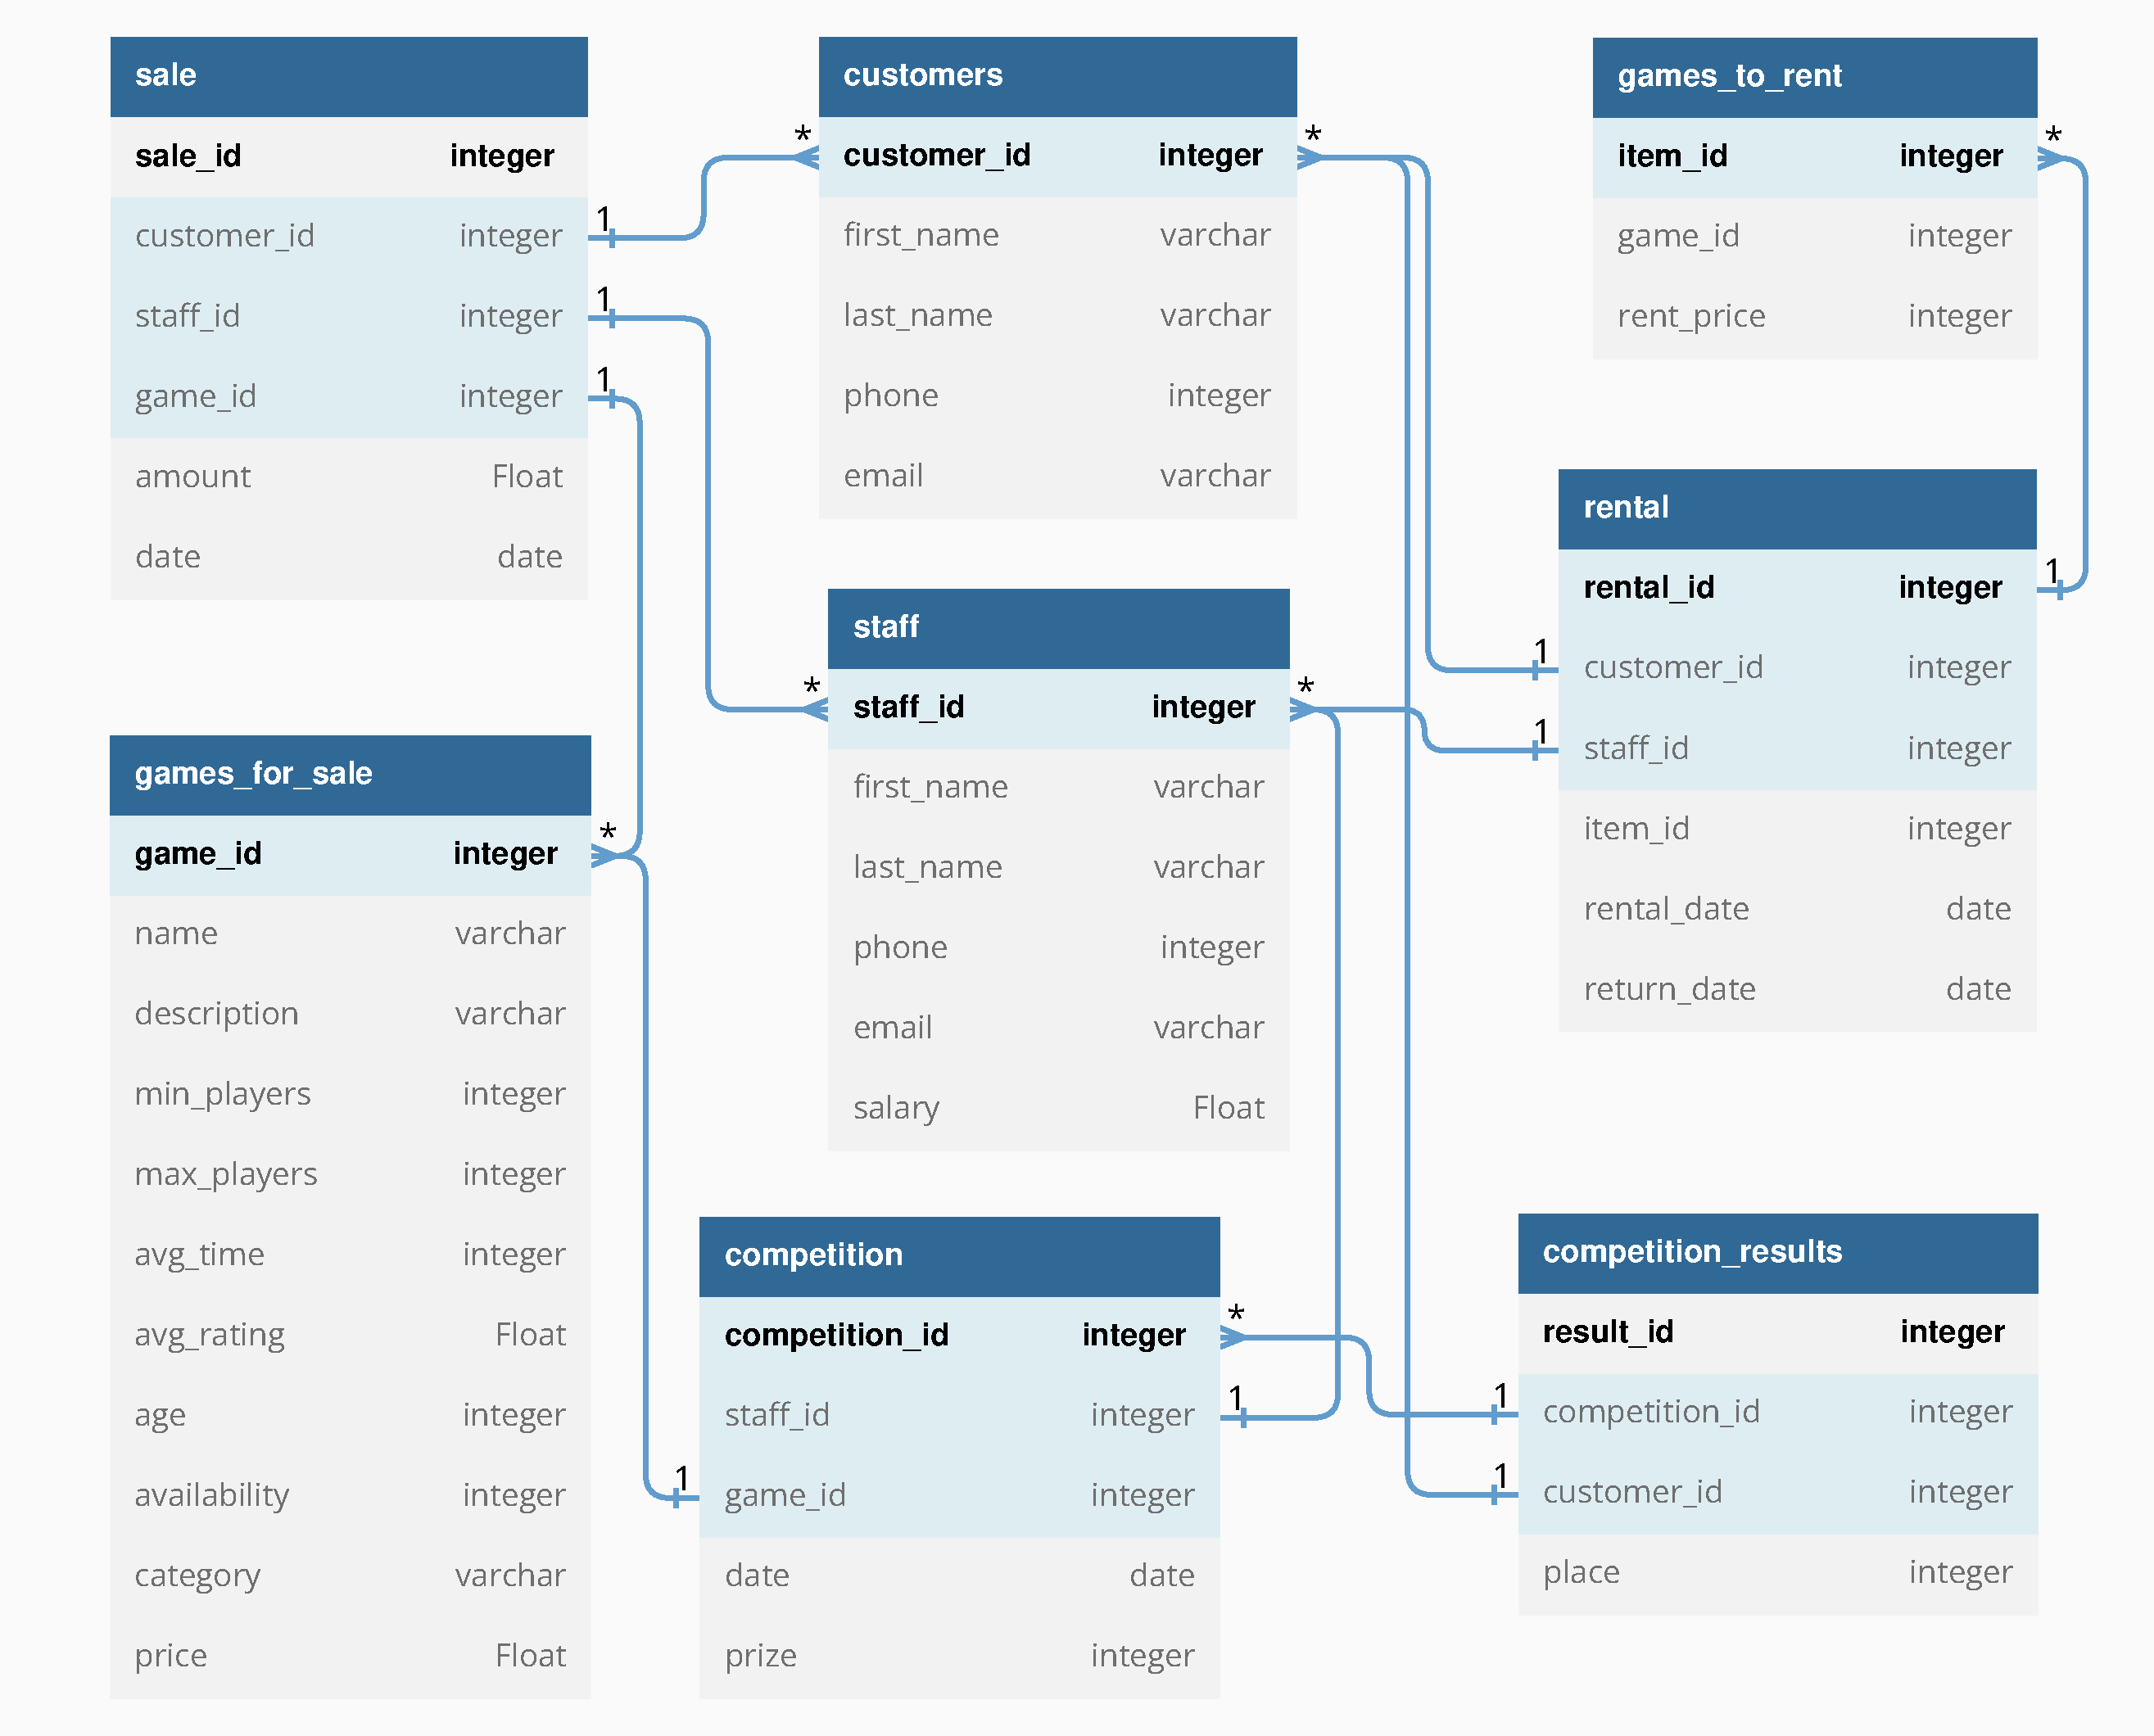
\includegraphics[width=13cm]{database_schema.pdf}
		\vspace{-0.6cm}
		\caption{Schemat bazy danych.}
	\end{figure}

	\section{Skryptowe wypełnienie bazy}
	
	W celu przygotowania do wypełnienia bazy losowo wygenerowanymi danymi, zostały stworzone pliki csv odpowiadające poszczególnym tabelom z bazy danych. Oprócz danych generowanych losowo, pojawiają się rownież dane rzeczywiste, co zostanie opisane w dalszej części tego rozdziału. Na sam koniec, po połączniu z serwerem, dane zostały zaimportowane do bazy.
	
	\subsection{Tabela customers}
		Tabela customers zawiera informacje na temat 1329 klientów, które zorganizowane są w  5 następujących kolumnach:
		\begin{itemize}
			\setlength{\itemsep}{-2pt}
			\item \textbf{cusomer\textunderscore id} – unikalne id dla każdego klienta,
			\item \textbf{first\textunderscore name} – imię klienta,
			\item \textbf{last\textunderscore name} – nazwisko klienta,
			\item \textbf{phone} – numer telefonu klienta,
			\item \textbf{email} – adres email klienta.
		\end{itemize}
		
		\noindent Dane w tabeli zostały wygenerowane w sposób losowy. Wartości w tabeli cusomer\textunderscore id wygenerowane zostały na pomocą odpowiedniego przedziału  dodatnich liczb całkowitych. Imiona i nazwiska klientów zostały wylosowane z odpowiednim prawdopodobieństwem korzystając z danych zamieszczonych na stronie \href{https://stat.gov.pl/}{Głównego Urzędu Statystycznego}. W pierwszej kolejności został wygenerowany wektor określający płeć klienta, z odpowiednim prawdopodobieństwem występowania danej płci, na podstawie liczby ludności we Wrocławiu z podziałem na mężczyzn i kobiety. Następnie w zależności od płci zostały przypisane imiona i nazwiska z odpowiednich tabeli danych pobranych ze wspomnianej strony internetowej.\\
		
		\noindent Następna kolumna zawiera losowo generowane numery kontaktowe klientów. Numer w każdym przypadku składa się z połączenia losowo wybieranego wyróżnika sieci telefonicznej (2 cyfry) oraz liczby z przedziału (1000000, 9000000). Lista dostępnych wyróżników została stworzona na podstawie informacji dostępnych na stronie \href{https://pl.wikipedia.org/wiki/Numery_telefoniczne_w_Polsce}{Wikipedii}. W~ten sposób uzyskaliśmy indywidualny 9-cyfrowy numer dla każdego klienta.\\
		
		\noindent Ostatnia kolumna zawiera adresy email, dla których identyfikatory użytkownika są generowane losowo na podstawie imion i nazwisk klientów. Identyfikatory adresów email składają się przykładowo:
		\begin{itemize}
			\setlength{\itemsep}{-2pt}
			\item z połączenia imienia i nazwiska lub części nazwiska klienta,
			\item z połączenia imienia lub nazwiska i losowej liczby z przedziału (100, 10000).
		\end{itemize}
	
		\noindent Każdy adres email składa się również z domeny, która była losowana z listy domen stworzonej na podstawie rankingu najpopularniejszych serwisów pocztowych w Polsce dostępnego na stronie \href{https://interaktywnie.com/biznes/artykuly/biznes/przeglad-ktora-poczta-e-mail-jest-najlepsza-16950}{interaktywnie.com}. Oczywiście, domeny były losowane z odpowiednim prawdopodobieństwem określonym według  liczby użytkowników korzystających z wybranych serwisów pocztowych.
		
	\subsection{Tabela staff}
		Tabela staff zawiera 6 kolumn z następującymi informacjami na temat 17 pracowników sklepu:
		\begin{itemize}
			\setlength{\itemsep}{-2pt}
			\item \textbf{staff\textunderscore id} – zawiera unikalne id dla każdego pracownika,
			\item \textbf{first\textunderscore name} – imię pracownika,
			\item \textbf{last\textunderscore name} – nazwisko pracownika,
			\item \textbf{phone} – numer telefonu pracownika,
			\item \textbf{email} – adres email pracownika,
			\item \textbf{salary} – miesięczne wynagrodzenie pracownika (cena brutto).
		\end{itemize}
	
		\noindent Dane w pierwszych 4 kolumnach zostały wygenerowane w sposób analogiczny jak w przypadku tabeli customers. Nastąpiła zmiana w generowaniu adresów email dla pracowników. Są one tworzone w~jednakowy sposób dla każdego pracownika – składają się z połączenia imienia i nazwiska za pomocą kropki oraz odrębnej domeny firmy @dragons.com.\\
		
		\noindent Ostatnia kolumna określa miesięczne wynagrodzenie pracownika, które były losowane z listy konkretnych pensji [4310, 5140, 6530, 7280, 8320], które zostały wybrane na podstawie możliwych zarobków na stanowiskach dotyczących obsługi klienta. Losowanie odbyło się z ustalonym prawdopodobieństwem, zakładającym, że doświadczonych pracowników o większych zarobkach jest mniej.
		
	\subsection{Tabela games\textunderscore for\textunderscore sale}
	Tabela \textbf{games\textunderscore for\textunderscore rent} zawiera podstawowe informacje dotyczące 3723 unikatowych gier nieelektronicznych. Są to kolejno:
	\begin{itemize}
		\setlength{\itemsep}{-2pt}
		\item \textbf{game\textunderscore id} - unikatowy identyfikator gry
		\item \textbf{name} - tytuł gry
		\item \textbf{description} - krótki opis gry
		\item \textbf{min\textunderscore players} - minimalna liczba graczy
		\item \textbf{max\textunderscore players} - maksymalna liczba graczy
		\item \textbf{avg\textunderscore time} - średni czas trwania rozgrywki
		\item  \textbf{avg\textunderscore rating} - średnia ocena gry
		\item \textbf{age} - minimalne ograniczenie wiekowe
		\item \textbf{availability} - ilość egzemplarzy dostępnych do sprzedaży
		\item  \textbf{category} - kategorie, do których zalicza się dana gra (może być więcej niż jedna kategoria)
		\item \textbf{price} - aktualna cena gry
		\item \textbf{rent\textunderscore price} - cena za wypożyczenie (dzienna)
	\end{itemize}
	
	\noindent Dane pochodzą z forum i sklepu internetowego \href{boardgamegeek.com}{boardgamegeek.com}, natomiast zostały one pobrane ze strony \href{https://www.kaggle.com/datasets/mrpantherson/board-game-data}{Kaggle}.
	Główną zmianą w oryginalnym zbiorze danych było usunięcie kolumn z danymi, których nie planowaliśmy brać pod uwagę. Ponadto rozszerzyliśmy ją o trzy dodatowe informacje: opis gry (description), cenę (price), oraz koszt wypożyczenia (rent\textunderscore price). \\ \\
	W celu wyciągnięcia informacji o cenie i opisie gry, zdecydowaliśmy się zbadać kod źródłowy każdej strony (kolumna bgg\textunderscore url z oryginalnej tabeli). Do tego zadania wykorzystaliśmy trzy bardzo istotne biblioteki: requests, BeautifulSoup, oraz Selenium, które dokładniej opisujemy w sekcji Technologie. Natomiast koszt wypożyczenia został wygenerowany następująco: grą których cena znajduje się w~określonym zakresie, przypisujemy odpowiednią cenę wypożyczenia:
	
	\begin{center}\centering
		\begin{tabular}{|c|c|c|}
			\hline
			\textbf{Cena produktu} & \textbf{Cena wypożyczenia}\\
			\hline
			$[0, 100)$ & $2$\\
			\hline
			$[100, 500)$ & $5$\\
			\hline
			$[500, 1000)$ & $10$\\
			\hline
			$[1000, 1500)$ & $15$\\
			\hline
			$>1500$ & $20$\\
			\hline
		\end{tabular}
	\end{center}
	
	
	
	\subsection{Tabela games\textunderscore to\textunderscore rent}
	Tabela gier do wypożycznia powstaje na podstawie tabeli games\textunderscore for\textunderscore sale wybieramy z niej jedynie kolumnę games\textunderscore id, a następnie dla każdego identyfikatora (czyli dla każdego tytułu gry) losujemy liczbę z przedziału [0, 10] (z pewną ustaloną przewagą zer). Wylosowana liczba będzie liczbą egzemplarzy przeznaczonych do wypożyczenia. Duplikujemy każdy wiersz o wylosowany numer i każdemu egzemplarzowi przypisujemy unikatowy identyfikator. Umieszczamy je w kolumnie item\textunderscore id.
	
	\subsection{Tabela sale}
		W tabeli znajduje się 6 kolumn:
		\begin{itemize}
			\setlength{\itemsep}{-2pt}
			\item \textbf{sale\textunderscore id} – unikalne id dla każdej sprzedaży,
			\item \textbf{customer\textunderscore id} – id klienta,
			\item \textbf{staff\textunderscore id} – id pracownika,
			\item \textbf{game\textunderscore id} – id gry,
			\item \textbf{amount} – kwota transakcji,
			\item \textbf{date} – data transakcji.
		\end{itemize}

		\noindent Dane w tabeli obejmują 117810 transakcji. Każda sprzedaż (wiersz w tabeli) była generowana w~następujący sposób:
		\begin{itemize}
			\setlength{\itemsep}{-2pt}
			\item customer\textunderscore id jest losowane z równym prawdopodobieństwem ze wszystkich dostępnych id klientów, a następnie z prawdopodobieństwem 0.83 zamieniane na NULL, co ma symulować klientów, którzy nie mają założonego konta w sklepie,
			\item staff\textunderscore id jest losowane z równym prawdopodobieństwem ze wszystkich dostęnych id pracowników,
			\item game\textunderscore id jest losowane z tabeli games\textunderscore for\textunderscore sale z prawdopodobieństwem proporcjonalnym do oceny gry (avg\textunderscore rating),
			\item amount to wartość price z tabeli games\textunderscore for\textunderscore sale powiększona o losową wartość proporcjonalną do tego, jak dawno transakcja miała miejsce (gra mogła być kiedyś droższa),
			\item date jest losowane spośród wszystkich dni pracujących od otwarcia sklepu do dziś z prawdopodobieństwem proporcjonalnym do czasu, jaki upłynął od otwarcia sklepu (sprzedaż rośnie wraz z czasem).
		\end{itemize}

	
	\subsection{Tabela rental}
        Tabela ta generowana jest podobnie do tabeli sale, z kilkoma różnicami. Jedną z nich jest to, że tutaj customer\textunderscore id już nie zawiera wartości NULL, ponieważ klient, by wypożyczyć grę, musi mieć założone konto. Nastepnie kolumna item\textunderscore id jest tworzona po wylosowaniu game\textunderscore id (ponownie opieramy się na avg\textunderscore rating) i dopasowaniu odpowiadającego mu item\textunderscore id. W przypadku kolumny return\textunderscore date losujemy czas wypożyczenia gry z rozkładu Poissona i dodajemy do rental\textunderscore date.

	
	\subsection{Tabela competition}

	Przechowuje ona ogólne informacje dotyczące turniejów. Zawiera 5 kolumn:
		
		\begin{itemize}
			\setlength{\itemsep}{-2pt}
			\item \textbf{competition\textunderscore id} – unikalne id dla każdego turnieju,
			\item \textbf{staff\textunderscore id} –  id prowadzącego turniej,
			\item \textbf{game\textunderscore id} – id gry turniejowej,
			\item \textbf{date} – data rozegrania turnieju,
			\item \textbf{prize} – pula nagród.
		\end{itemize}

	\noindent Turnieje rozgrywane są co piątek z wyłączeniem dni ustawowo wolnych od pracy oraz Wielkiego Piątku. Aby wziąć udział w turnieju, gracz musi posiadać konto. Spośród stałych klientów losujemy trzydziestu graczy. Jako prowadzący przypisany jest losowo wybrany pracownik wypożyczalni. Losowa jest także nagroda za dany turniej. Nie w każdym wydarzeniu biorą udział wszyscy zadeklarowani. Graczy nie może być mniej niż minimalna oraz nie może przekraczać trzykrotności maksymalnej ilości graczy dla danej gry. Gry turniejowe wybierane są losowo spośród dwudziestu najlepiej ocenianych gier, a daty przypisywane są na cały rok kalendarzowy.
	
	\subsection{Tabela competition\textunderscore results}

	Tabela ta zawiera szczegółowe informacje dotyczące wyników w turnieju każdego uczestnika . Zawiera 4 kolumny:

		\begin{itemize}
			\setlength{\itemsep}{-2pt}
			\item \textbf{competition\textunderscore id} – id turnieju,
			\item \textbf{customer\textunderscore id} – id ,
			\item \textbf{place} – miejsce w turnieju,
			\item \textbf{result\textunderscore id} – unikalne id wyniku,
		\end{itemize}
	Miejsca zajmowane przez uczestników są losowe. 

	\subsection{Połączenie z bazą}
	Za połączenie z bazą oraz wypełnienie jej wygenerownymi danymi odpowiada plik Connection.py. Przesłanie danych do bazy możliwe jest dzięki bibliotece SQLAlchemy, która napisana jest w języku programowania Python i służy do pracy z bazami danych oraz mapowania obiektowo-relacyjnego.\\
	
	
	\noindent W pierwszej kolejności tworzymy obiekt Base, za pomocą funkcji declarative\textunderscore base(), który jest klasą bazową. Następnie, dla każdej z tabel bazy, tworzymy klasą dziedziczącą z klasy podstawowej Base. W następnym kroku, za pomocą funkcji create\textunderscore engine(), zapisujemy do zmiennej engine połączenie z~konkretną bazą. Dalej z wywołaniem funkcji Base.metadata.create\textunderscore all(engine) generowane są puste tabele bazy danych. Na sam koniec, z racji zapisywania generowanych danych losowych do tabel z~wykorzystaniem biblioteki pandas, ponownie jest ona wykorzystywana i za pomocą funkcji to\textunderscore sql() tabele wypelniane są odpowiednimi danymi.
	
	
	
	\section{Analiza danych i generowanie raportu}
	
	Raport został napisany w języku R Markdown z wykorzystaniem Pythona. W pliku Raport.rmd znajduje się kod którego przekompilowanie zwraca plik pdf. Raport jest napisany tak by był uniwersalny i~dostosowywał się do zmian w bazie danych. Plik rmd zawiera w sobie kod pythonowy, który w trakcie kompilacji pobiera z bazy dane i na ich podstawie tworzy wykresy i wylicza poszczególne statystyki.\\

	\noindent Raport odpowiada na następujące pytania i zagadnienia:
	\begin{itemize}
		\item Ranking na pracownika miesiąca.
		\item Ranking zawodników turniejowych.
		\item Które gry przynoszą największy dochód ze sprzedaży, a które z wypożyczeń?
		\item Które kategorie są najpopularniejsze?
		\item Jak zmieniała się sprzedaż na przestrzeni lat?
		\item Czy ocena gry i cena wpływają na sprzedaż?
		\item Ile gier dostępne jest w sklepie?
	\end{itemize}



	
	\section{Technologie}
	Poniżej znajduję się spis technologii wykorzystywanych podczas pracy nad projektem, których użycie było wspominane w niniejszej dokumenatcji. Dla każdej pozycji jest dołączony link do dokumnetacji.
	\begin{itemize}
		\setlength{\itemsep}{-2pt}
		\item MariaDB (\href{https://mariadb.com/kb/en/}{dokumntacja})
		\item Python (\href{https://www.python.org/doc/}{dokumntacja})
		\item SQLAlchemy (\href{https://www.sqlalchemy.org/}{dokumntacja})
		\item Selenium (\href{https://selenium-python.readthedocs.io/?fbclid=IwAR3mhY42CU1bHhruIm0kzWo9hTZjRoGbooMU2BGEkrFJWPC9i9e93pRitqY}{dokumntacja})
		\item BeautifulSoup (\href{https://beautiful-soup-4.readthedocs.io/en/latest/}{dokumntacja})
		\item RMarkdown (\href{https://www.rdocumentation.org/packages/rmarkdown/versions/2.22}{dokumntacja})
		\item Reticulate (\href{https://rstudio.github.io/reticulate/}{dokumntacja})
	\end{itemize}
	
	
	
	\section{Zarządzanie plikami}
	Cały proces generowania danych i łączenia z bazą oraz analizy i generowania raportu został tak zorganizowany w plikach, aby mógł być odtworzony w bardzo łatwy sposób. Poniżej przedstawiona jest lista plików wraz z opisem ich zawartości:
	\begin{itemize}
		\setlength{\itemsep}{-2pt}
		\item \textbf{Data\textunderscore generation.py} – Plik generuje dane to tabel w pandas, które następnie zapisuje do plików csv w~folderze database.
		\item \textbf{Connection.py} – Plik łączy się z bazą oraz wczytuje dane z~plików csv znajdujących się w~folderze database do tabel w pandas.
		Następnie tabele te przesyła do bazy z~wykorzystaniem biblioteki SQLAlchemy.
		\item \textbf{Raport.rmd} – Plik generuje raport z analizą danych.	
	\end{itemize}
	
	
	\noindent Aby uzyskać gotowy projekt, należy najpierw utworzyć w folderze głównym plik tekstowy o nazwie python\textunderscore path.txt i wpisać w nim ściężkę do pythona na swoim komputerze. Następnie należy w~następującej kolejności uruchomić wymionione powyżej pliki:
	\begin{enumerate}
		\setlength{\itemsep}{-2pt}
		\item Data\textunderscore generation.py
		\item Connection.py
		\item Raport.rmd
	\end{enumerate}

	Dodatkowo w folderze data znajduje się description_and_price.py, który posłużył do rozszerzenia danych z grami o ich opis oraz cenę. Skrypt pythonowy zawarty w pliku łączy się ze stroną ..., skąd ściąga opisy gier, a nastepnie po połączeniu ze stroną ..., sciąga ceny gier. Tak uzyskane dane program dołącza do zbioru gier. W folderze data znajduje się już zbiór zawierający te kolumny, wiec kompilowanie tego pliku nie jest wymagane.
	
	\section{Baza w postaci EKNF}
	W tej części dokumentacji zawarto listę zależności funkcyjnych dla każdej relacji oraz uzasadnienie, że baza jest w EKNF.
	
	\paragraph{Tabela games\textunderscore for\textunderscore sale}\mbox{}\vspace{0.2cm} \\
	Zależność funkcyjna: \textbraceleft game\textunderscore id, name, description\textbraceright \mbox{} \textrightarrow \mbox{} pozostałe kolumny \vspace{0.2cm} \\
	\noindent Uzasadnieniem jest fakt, że game\textunderscore id jest kluczem głównym tabeli, a name i description są wartościami unikalnymi dla każdego game\textunderscore id, więc każda pozostała kolumna zależy funkcyjnie od zbioru tych trzech atrybutów. Jest to więc nietrywialna zależność funkcyjna, która zaczyna się od nadklucza, a więc nie zaburza to postaci EKNF bazy.

	\paragraph{Tabela games\textunderscore to\textunderscore rent}\mbox{}\vspace{0.2cm} \\
	Zależność funkcyjna: item\textunderscore id\mbox{} \textrightarrow \mbox{} game\textunderscore id \vspace{0.2cm} \\
	\noindent Uzasadnieniem jest fakt, że item\textunderscore id jest kluczem głównym tabeli, więc game\textunderscore id zależy funkcyjnie od niego. Relacja ta nie zaburza postaci EKNF bazy, ponieważ tabela games\textunderscore to\textunderscore rent nie posiada żadnych niekluczowych zależności funkcyjnych.
	
	\paragraph{Tabela sale}\mbox{}\vspace{0.2cm} \\
	Zależność funkcyjna: sale\textunderscore id\mbox{} \textrightarrow \mbox{} pozostałe kolumny \vspace{0.2cm} \\
	\noindent Uzasadnieniem jest fakt, że sale\textunderscore id jest kluczem głównym tabeli, więc każda pozostała kolumna zależy funkcyjnie od niego. Relacja ta nie zaburza postaci EKNF bazy, ponieważ tabela games\textunderscore to\textunderscore rent nie posiada żadnych niekluczowych zależności funkcyjnych.
	
	\paragraph{Tabela rental}\mbox{}\vspace{0.2cm} \\
	Zależność funkcyjna: rental\textunderscore id\mbox{} \textrightarrow \mbox{} pozostałe kolumny \vspace{0.2cm} \\
	\noindent Uzasadnieniem jest fakt, że sale\textunderscore id jest kluczem głównym tabeli, więc każda pozostała kolumna zależy funkcyjnie od niego. Relacja ta nie zaburza postaci EKNF bazy, ponieważ tabela games\textunderscore to\textunderscore rent nie posiada żadnych niekluczowych zależności funkcyjnych.
	
	\paragraph{Tabela customers}\mbox{}\vspace{0.2cm} \\
	Zależność funkcyjna: \textbraceleft customer\textunderscore id phone, email\textbraceright \mbox{} \textrightarrow \mbox{} pozostałe kolumny \vspace{0.2cm} \\
	\noindent Uzasadnieniem jest fakt, że customer\textunderscore id jest kluczem głównym tabeli, a phone i email są wartościami unikalnymi dla każdego customer\textunderscore id, więc każda pozostała kolumna zależy funkcyjnie od zbioru tych trzech atrybutów. Jest to więc nietrywialna zależność funkcyjna, która zaczyna się od nadklucza, a~więc nie zaburza to postaci EKNF bazy.
	
	\paragraph{Tabela staff}\mbox{}\vspace{0.2cm} \\
	Zależność funkcyjna: \textbraceleft staff\textunderscore id phone, email\textbraceright \mbox{} \textrightarrow \mbox{} pozostałe kolumny \vspace{0.2cm} \\
	\noindent Uzasadnieniem jest fakt, że staff\textunderscore id jest kluczem głównym tabeli, a phone i email są wartościami unikalnymi dla każdego staff\textunderscore id, więc każda pozostała kolumna zależy funkcyjnie od zbioru tych trzech atrybutów. Jest to więc nietrywialna zależność funkcyjna, która zaczyna się od nadklucza, a~więc nie zaburza to postaci EKNF bazy.
	
	\paragraph{Tabela competition}\mbox{}\vspace{0.2cm} \\
	Zależność funkcyjna: competition\textunderscore id\mbox{} \textrightarrow \mbox{} pozostałe kolumny \vspace{0.2cm} \\
	\noindent Uzasadnieniem jest fakt, że competition\textunderscore id jest kluczem głównym tabeli, więc każda pozostała kolumna zależy funkcyjnie od niego. Relacja ta nie zaburza postaci EKNF bazy, ponieważ tabela games\textunderscore to\textunderscore rent nie posiada żadnych niekluczowych zależności funkcyjnych.
	
	\paragraph{Tabela competition\textunderscore results}\mbox{}\vspace{0.2cm} \\
	Zależność funkcyjna: result\textunderscore id\mbox{} \textrightarrow \mbox{} pozostałe kolumny \vspace{0.2cm} \\
	\noindent Uzasadnieniem jest fakt, że result\textunderscore id jest kluczem głównym tabeli, więc każda pozostała kolumna zależy funkcyjnie od niego. Relacja ta nie zaburza postaci EKNF bazy, ponieważ tabela games\textunderscore to\textunderscore rent nie posiada żadnych niekluczowych zależności funkcyjnych.\\
	
	\noindent Podsumowując, baza jest w EKNF, ponieważ każda z występujących w niej relacji nie zaprzecza tej postaci.
	
	\section{Podsumowanie}
	W dokumentacji został przedstawiony proces tworzenia bazy danych sklepu Geeks \& Dragons od momentu tworzenia schemtu bazy, aż po analizę wykonywaną na stworzonej bazie. Przebieg powstawania bazy został podzielowny na poszczególne etapy, co ułatwiło rodzielenie zadań pośród członków grupy zajmującej sie projektem. Najtrudniejszym zadaniem podczas realizacji projektu było przede wszystkim zrozumienie i uzasadnienie, że stworzona baza jest w  postaci EKNF. Ostatecznie grupa projektowa jest bardzo zadowolona z~efektów końcowych i ma nadzieje na wysoką, w domyśle możliwie najwyższą, punktacje za wykonane zadanie.
	
\end{document}